\chapter{Hardware Realization} \label{sec:hwreal}

\section{GEX on a STM32 Discovery Board}

It has been proposed earlier in the text that STM32 Nucleo and Discovery development boards might serve as the hardware platform for this project. Indeed, a Discovery board with the STM32F072 was used to develop a major part of the GEX firmware, and the firmware remains compatible with it. This inexpensive board may be used to try GEX without any custom hardware.

\subsection{Discovery STM32F072 Configuration and Pin Mapping}

The Discovery board is fitted with four \glspl{LED} on \gls{GPIO} pins PC6 through PC9, in a compass arrangement. The ``north'' \gls{LED}, PC6, is used as the status indicator. The ``User'' button, connected to PA0, is mapped as the Lock button, controlling the settings storage.

We advise the reader, as a potential user of the board, to review its schematic diagram (found in the documentation~\cite{disco-f072}) and ensure the solder-jumpers on the back side are configured correctly:

\begin{itemize}
	\item Jumpers SB20 and SB23 must be closed to enable the User \gls{USB} connector.
	
	\item Jumper SB17 must be open and SB19 closed to use the 8\,MHz clock signal provided by the on-board ST-Link programmer; the internal USB-synchronized 48\,MHz oscillator will be used if the clock signal is not provided (SB19 open).
	
	\item Jumpers SB27 through SB32 should be closed to connect the \gls{GPIO} pins normally dedicated to the touch sensing strip to the board's header.
\end{itemize} 

Capacitors C26, C27, and C28 are sampling capacitors for the \gls{TSC}. There are, unfortunately, no jumpers available to disconnect them, and they interfere in high-speed signals on the used pins (PA3, PA7, and PB1). The only solution, when those pins are needed for another purpose, is to desolder the capacitors.

An accelerometer \gls{IC} L3GD20 is fitted on the board, attached to SPI2 on pins PB13 (\gls{SCK}), PB14 (\gls{MISO}), and PB15 (\gls{MOSI}), with \gls{NSS} on pin PC0, and pins PC1 and PC2 used for interrupt flags. This chip cannot be disconnected or disabled and it is difficult to remove; care must be taken to avoid its interference on the used pins.

\section{GEX Hub}

GEX Hub was the first custom \gls{PCB} designed for GEX. It uses the same microcontroller as the Discovery board, thus the firmware modifications needed to make it work with this new platform were minimal. The schematic diagram is attached in \hyperref[apx:gex_hub]{Appendix A}.

The Hub board provides access to all the \gls{GPIO} pins\footnote{With the exception of pins used by USB and the Lock button.} through three flat-cable connectors (IDC), one for each port; they also contain a ground and power supply connection to make the attachment of external boards or a breadboard easier, requiring just one cable. The use of flat cables, however, is not mandatory---the flat cable connectors are based on the standard 2.54\,mm-pitch pin headers, allowing the user to use widely available ``jumper wires''.

\begin{figure}[h]
	\centering
	\begin{subfigure}{.5\textwidth}
		\centering
		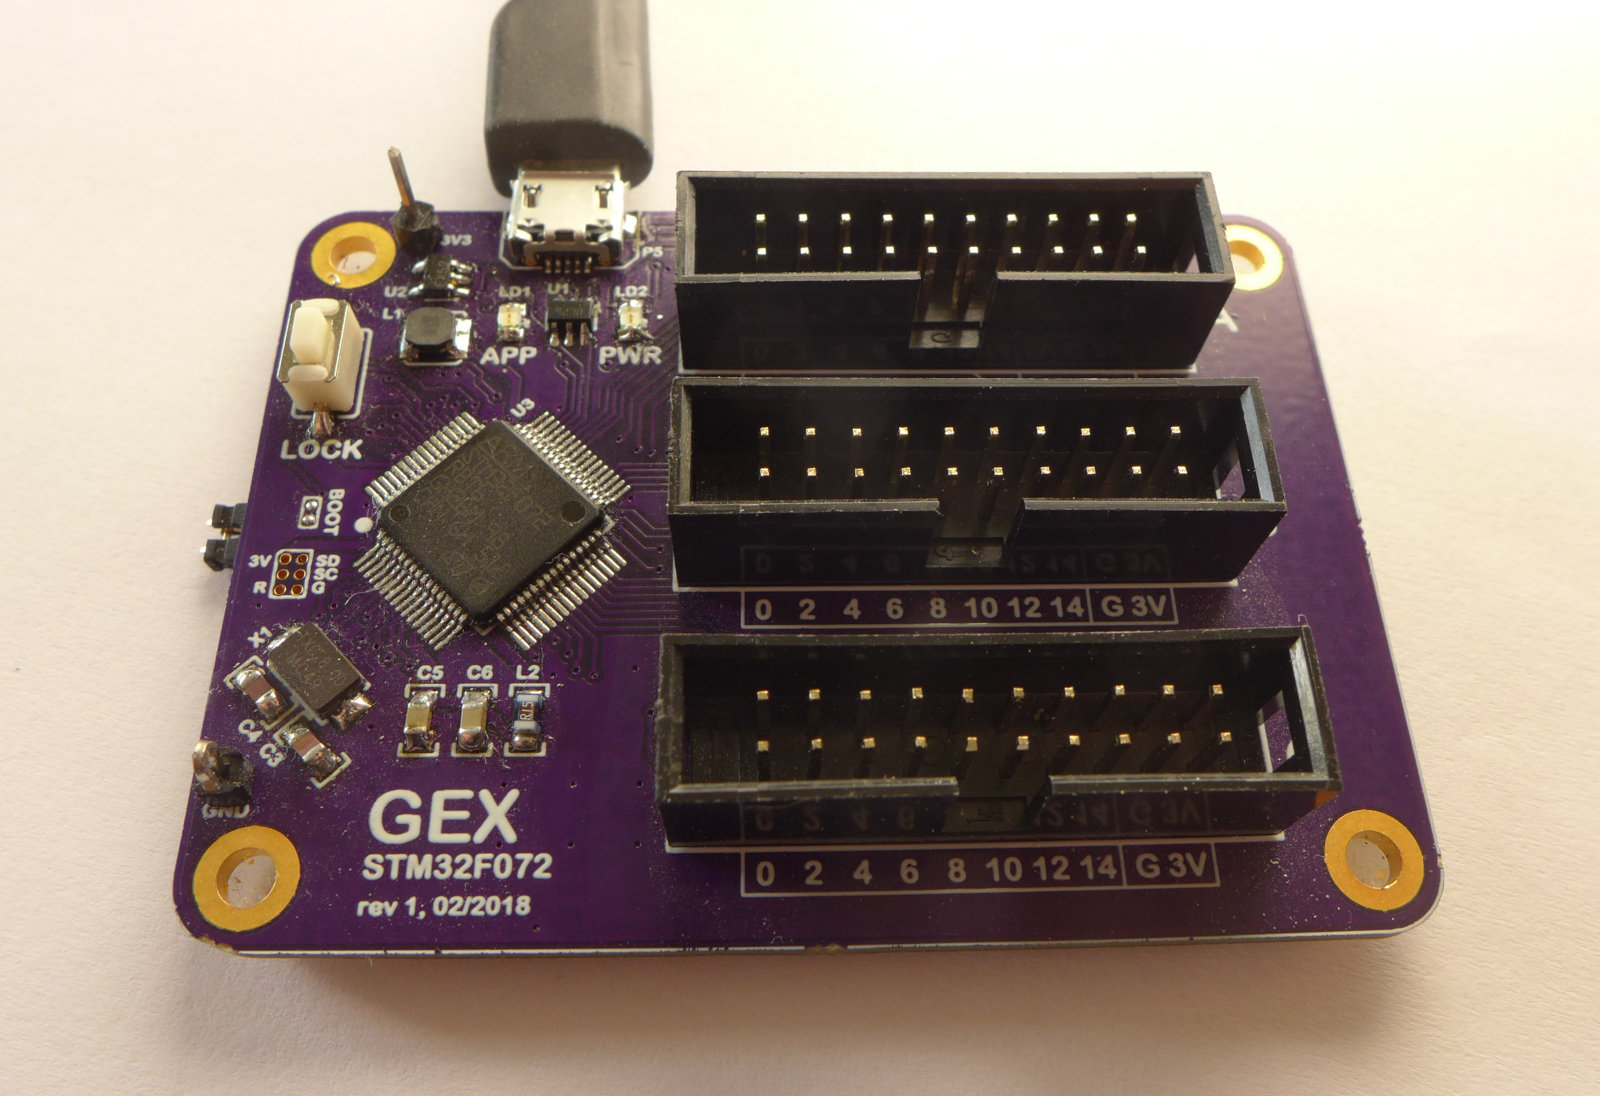
\includegraphics[width=.98\linewidth]{img/photo-hub1.jpg}
		\caption{\label{fig:gexhub1}Revision 1}
	\end{subfigure}%
	\begin{subfigure}{.5\textwidth}
		\centering
		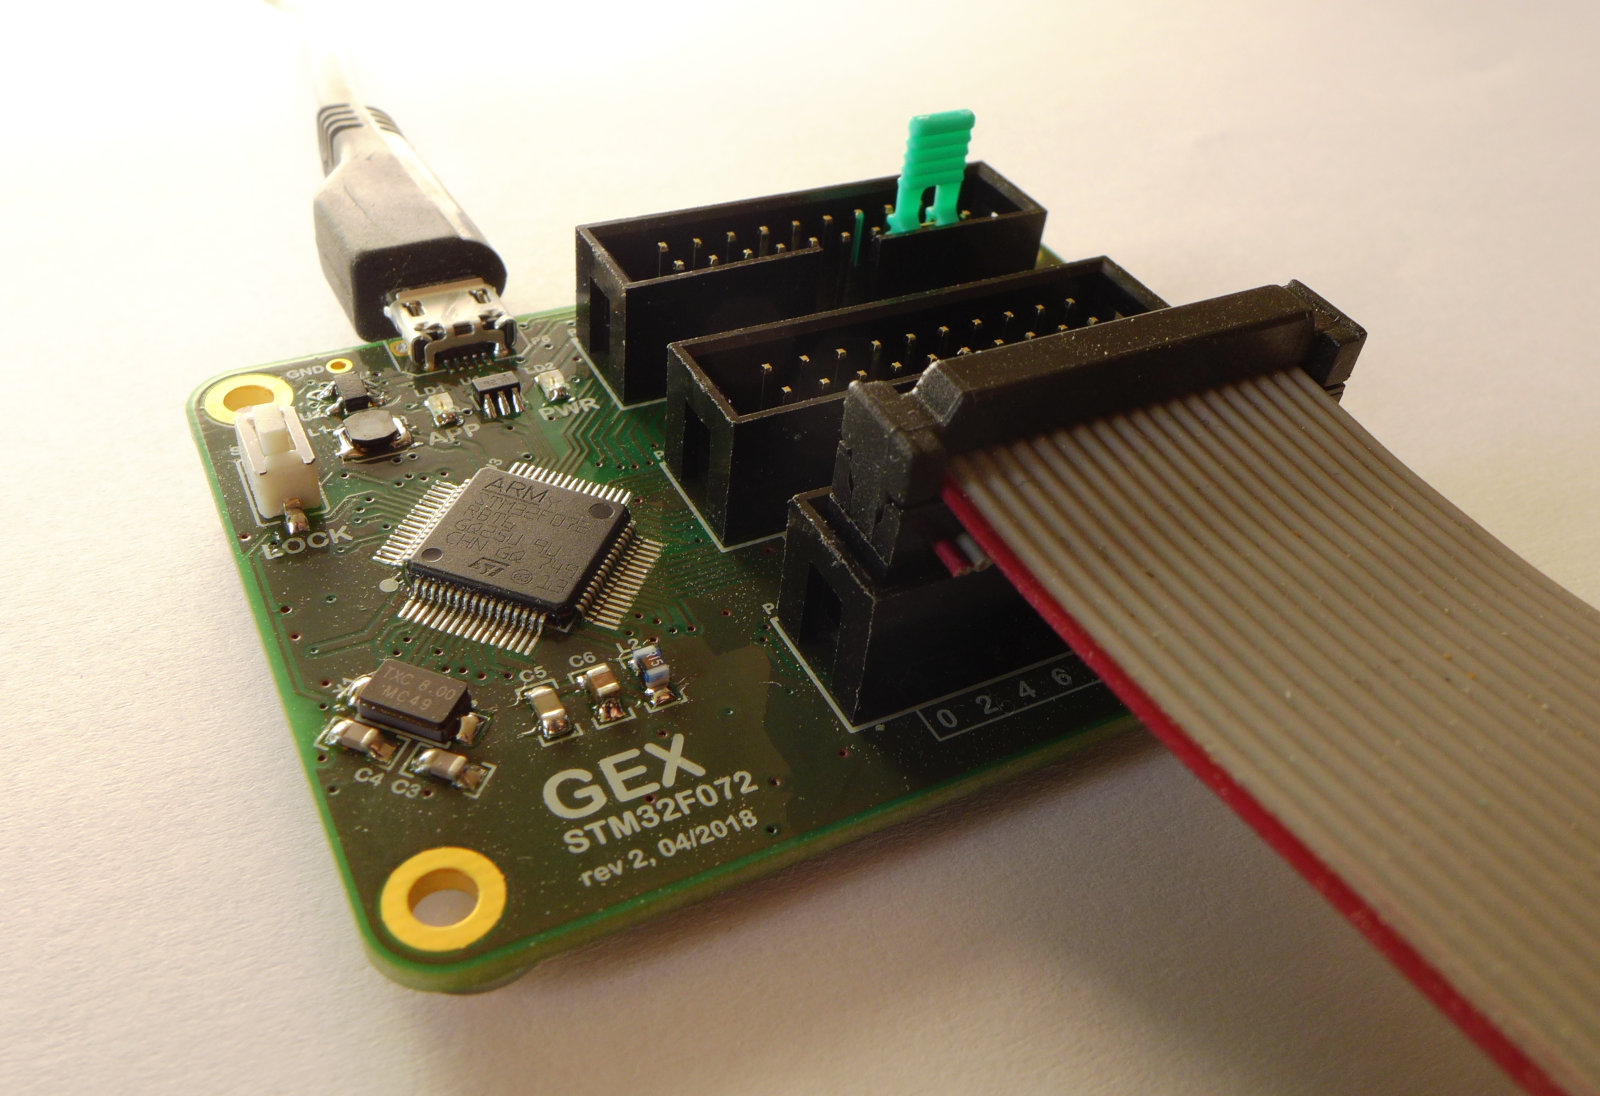
\includegraphics[width=.98\linewidth]{img/photo-hub2.jpg}
		\caption{\label{fig:gexhub2}Revision 2}
	\end{subfigure}
	\caption[The GEX Hub module]{\label{fig:gexhub} Two revisions of the GEX Hub module, rev. 2 shown with the boot jumper and one flat cable.}
\end{figure}

\subsection{GEX Hub Errata}

The first revision of the Hub board (\cref{fig:gexhub1}) proved functional and helped us validate the power supply design and test the firmware, but contained one layout error that had to be manually fixed---the boot jumper and the programming header footprints, on the left side of the board, had too fine pitch and could not be populated.

An updated revision 2 of the board (\cref{fig:gexhub2}), manufactured together with the GEX Zero \glspl{PCB} (\cref{sec:gzero}), removes the two problematic footprints altogether; a reorganization in the \gls{GPIO} connectors allowed them to be moved together with the other pins. 

The Boot jumper was meant to be closed during normal operation, to avoid it getting lost. Since revision 2 moved the boot pin into the top connector, this had to be changed; the jumper logic was inverted by changing its pull-up resistor to a pull-down. The bootloader is now activated by inserting a jumper into the connector, shorting the Boot pin (labeled ``B'') to the adjacent 3.3\,V pin.

A restart is required, in all cases, for the boot jumper changes to take effect. Revision 2 adds a flat reset button on the back side of the board for this purpose, making the firmware update process more straightforward.

\begin{figure}[h]
	\centering
	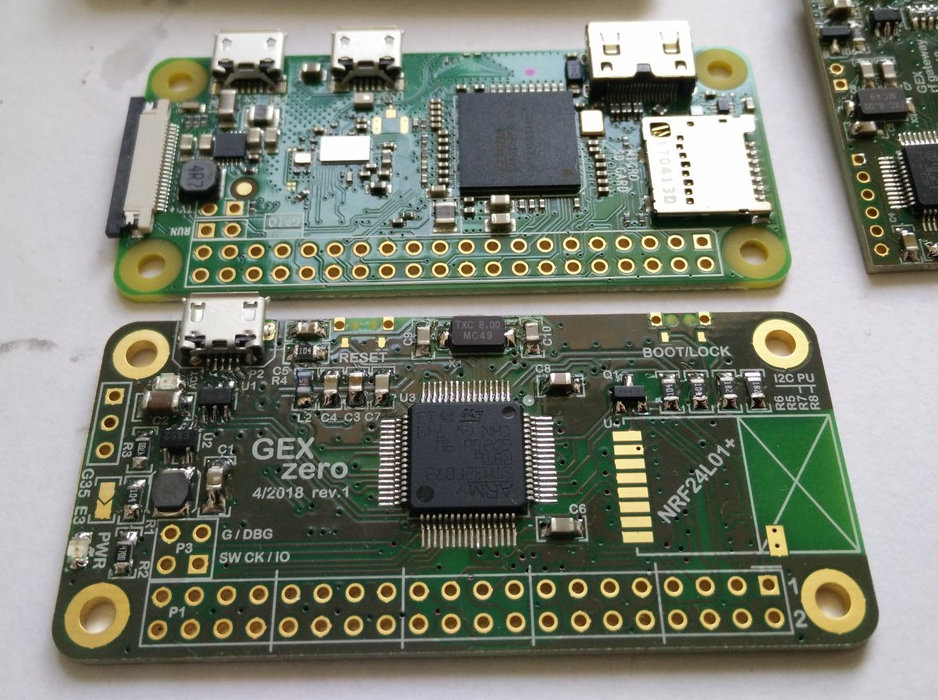
\includegraphics[width=.9\textwidth]{img/photo-zero-pi-compare.jpg}
	\caption[GEX Zero compared to Raspberry Pi Zero]{\label{fig:zpicompare}Comparison of Raspberry Pi Zero (top) with GEZ Zero (bottom), before soldering the header, buttons, and the wireless module.}
\end{figure}

\begin{figure}[h]
	\centering
	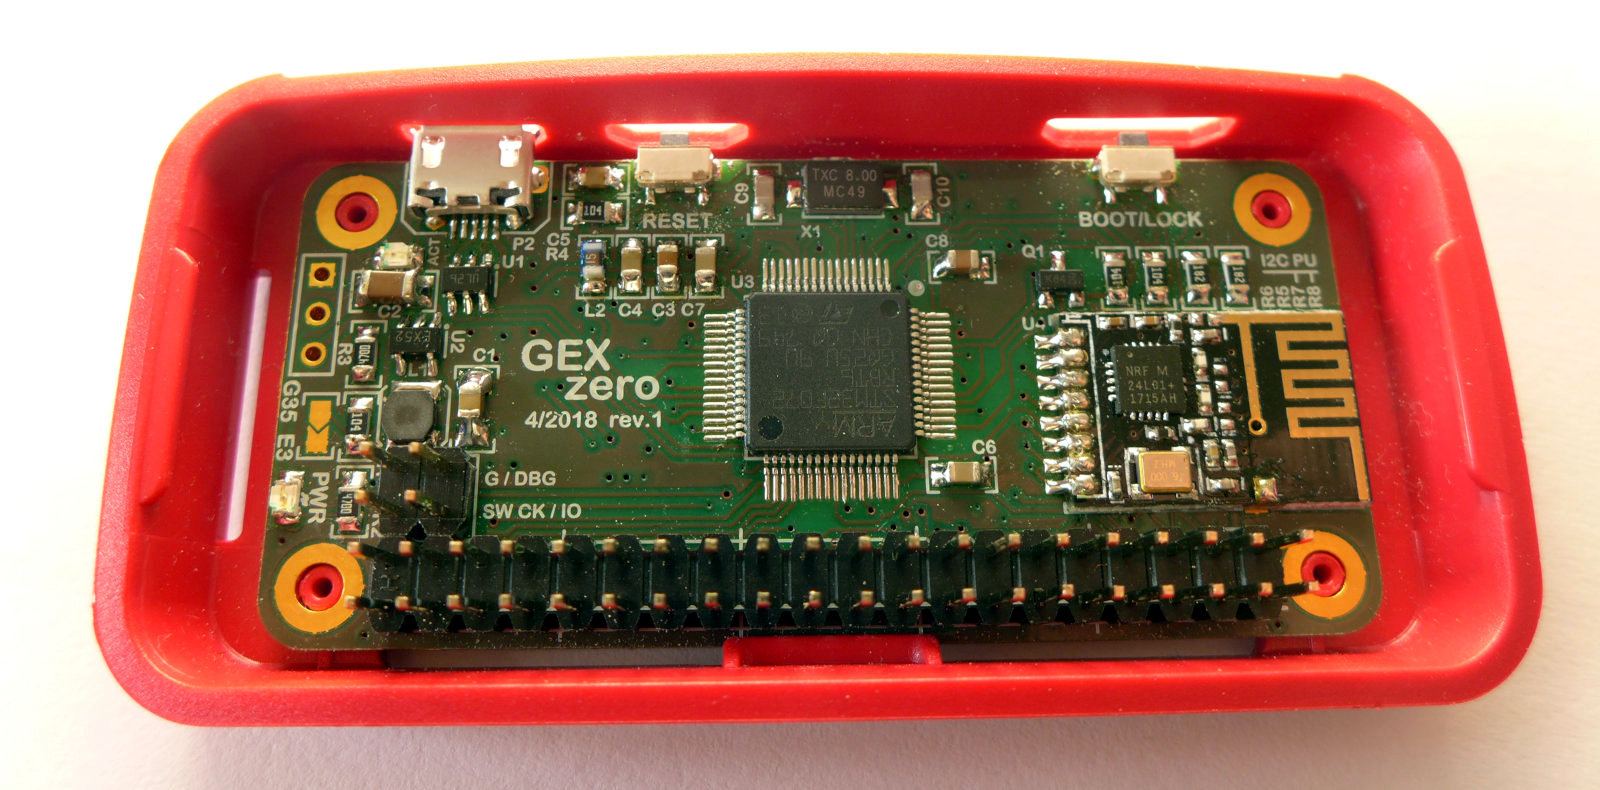
\includegraphics[width=.85\textwidth]{img/photo-zero-picase.jpg} \\
	\vspace{1mm}
	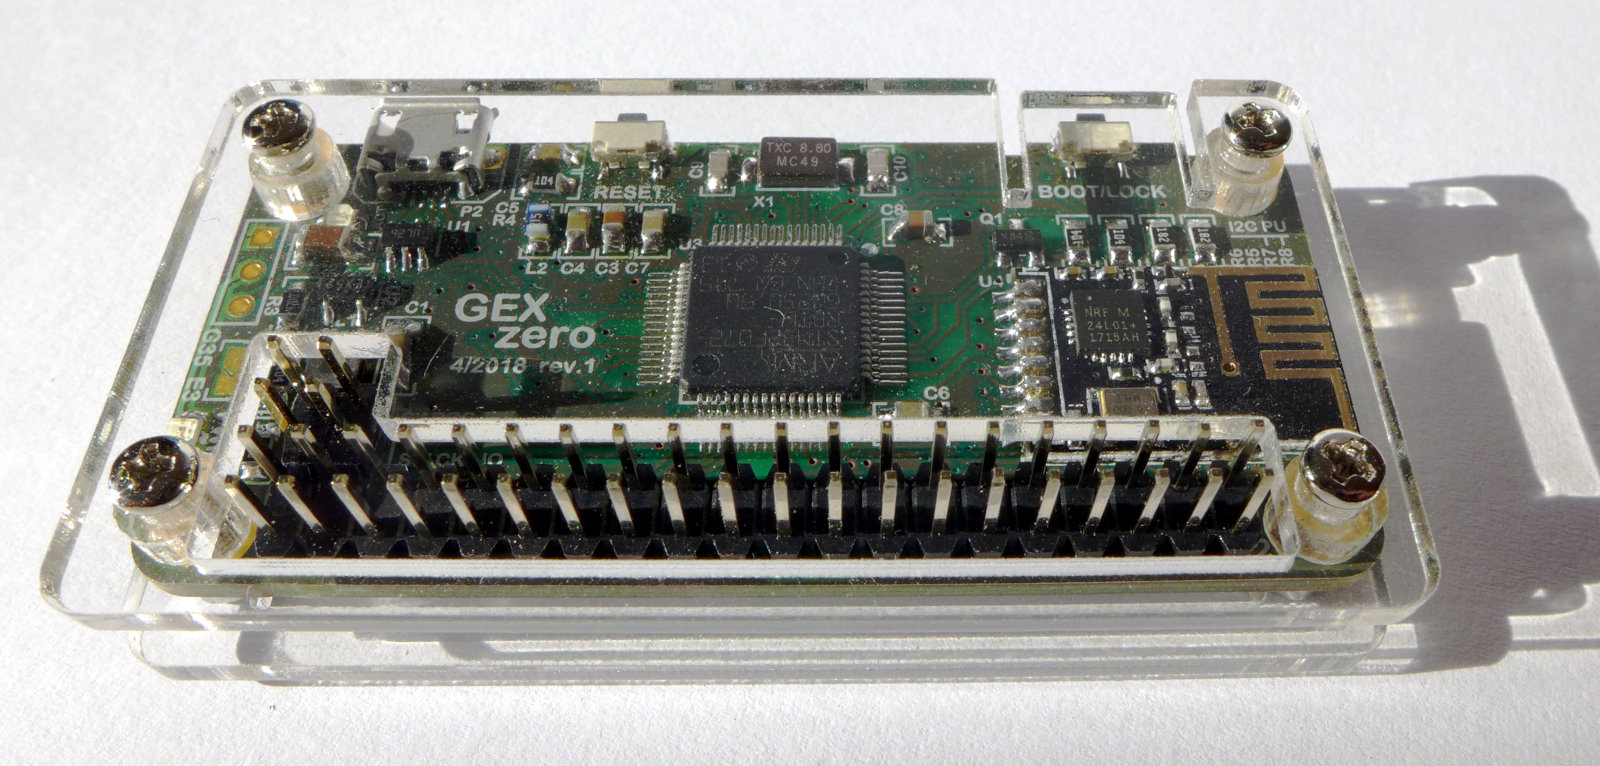
\includegraphics[width=.85\textwidth]{img/photo-zero-transparent.jpg}
	\caption[The GEX Zero module]{\label{fig:gexzcases}GEX Zero in the official Raspberry Pi Zero case, and an aftermarket acrylic case. The acrylic case is a better choice, as the button and the side connector are easier accessible, and the pin-out diagram on the back side of the board can be read without removing it.}
\end{figure}

\section{GEX Zero}\label{sec:gzero}

Our desire to re-use the form factor of the Raspberry Pi (RPi) Zero to exploit the existing accessory market has been mentioned already in \cref{sec:formfactors}. It was brought to fruition with GEX Zero, the second realized GEX prototype (\cref{fig:gexzcases}). Its design involved several challenges given by constraints imposed by this form factor:

\begin{itemize}
	\item It had to be a one-sided board, with no components on the bottom; this is needed for acrylic cases which sit flatly against the \gls{PCB}, with a cut-out for the pin header.
	\item Buttons and the USB connector had to exactly align with connectors on the RPi Zero to fit the openings in its cases.
	\item The board size was fixed, and rather small; we used only two layers to save production cost, but this proved a significant challenge when routing connections to the pin header.
	\item To make use of the Raspberry Pi add-on boards, called HATs or pHATs, a particular organization of the pin header was required. We will discuss this in more detail below.
\end{itemize}

\subsection{Pin Assignment}

Like our STM32 microcontroller, the Broadcom processor on the RPi multiplexes its \gls{GPIO} pins with alternate functions, and, likewise, each function is available only on a small selection of pins. The usual alternate function assignments of the RPi \gls{GPIO} header can be found in~\cite{piheader} and~\cite{piheaderxyz}.

\begin{figure}[h]
	\centering
	%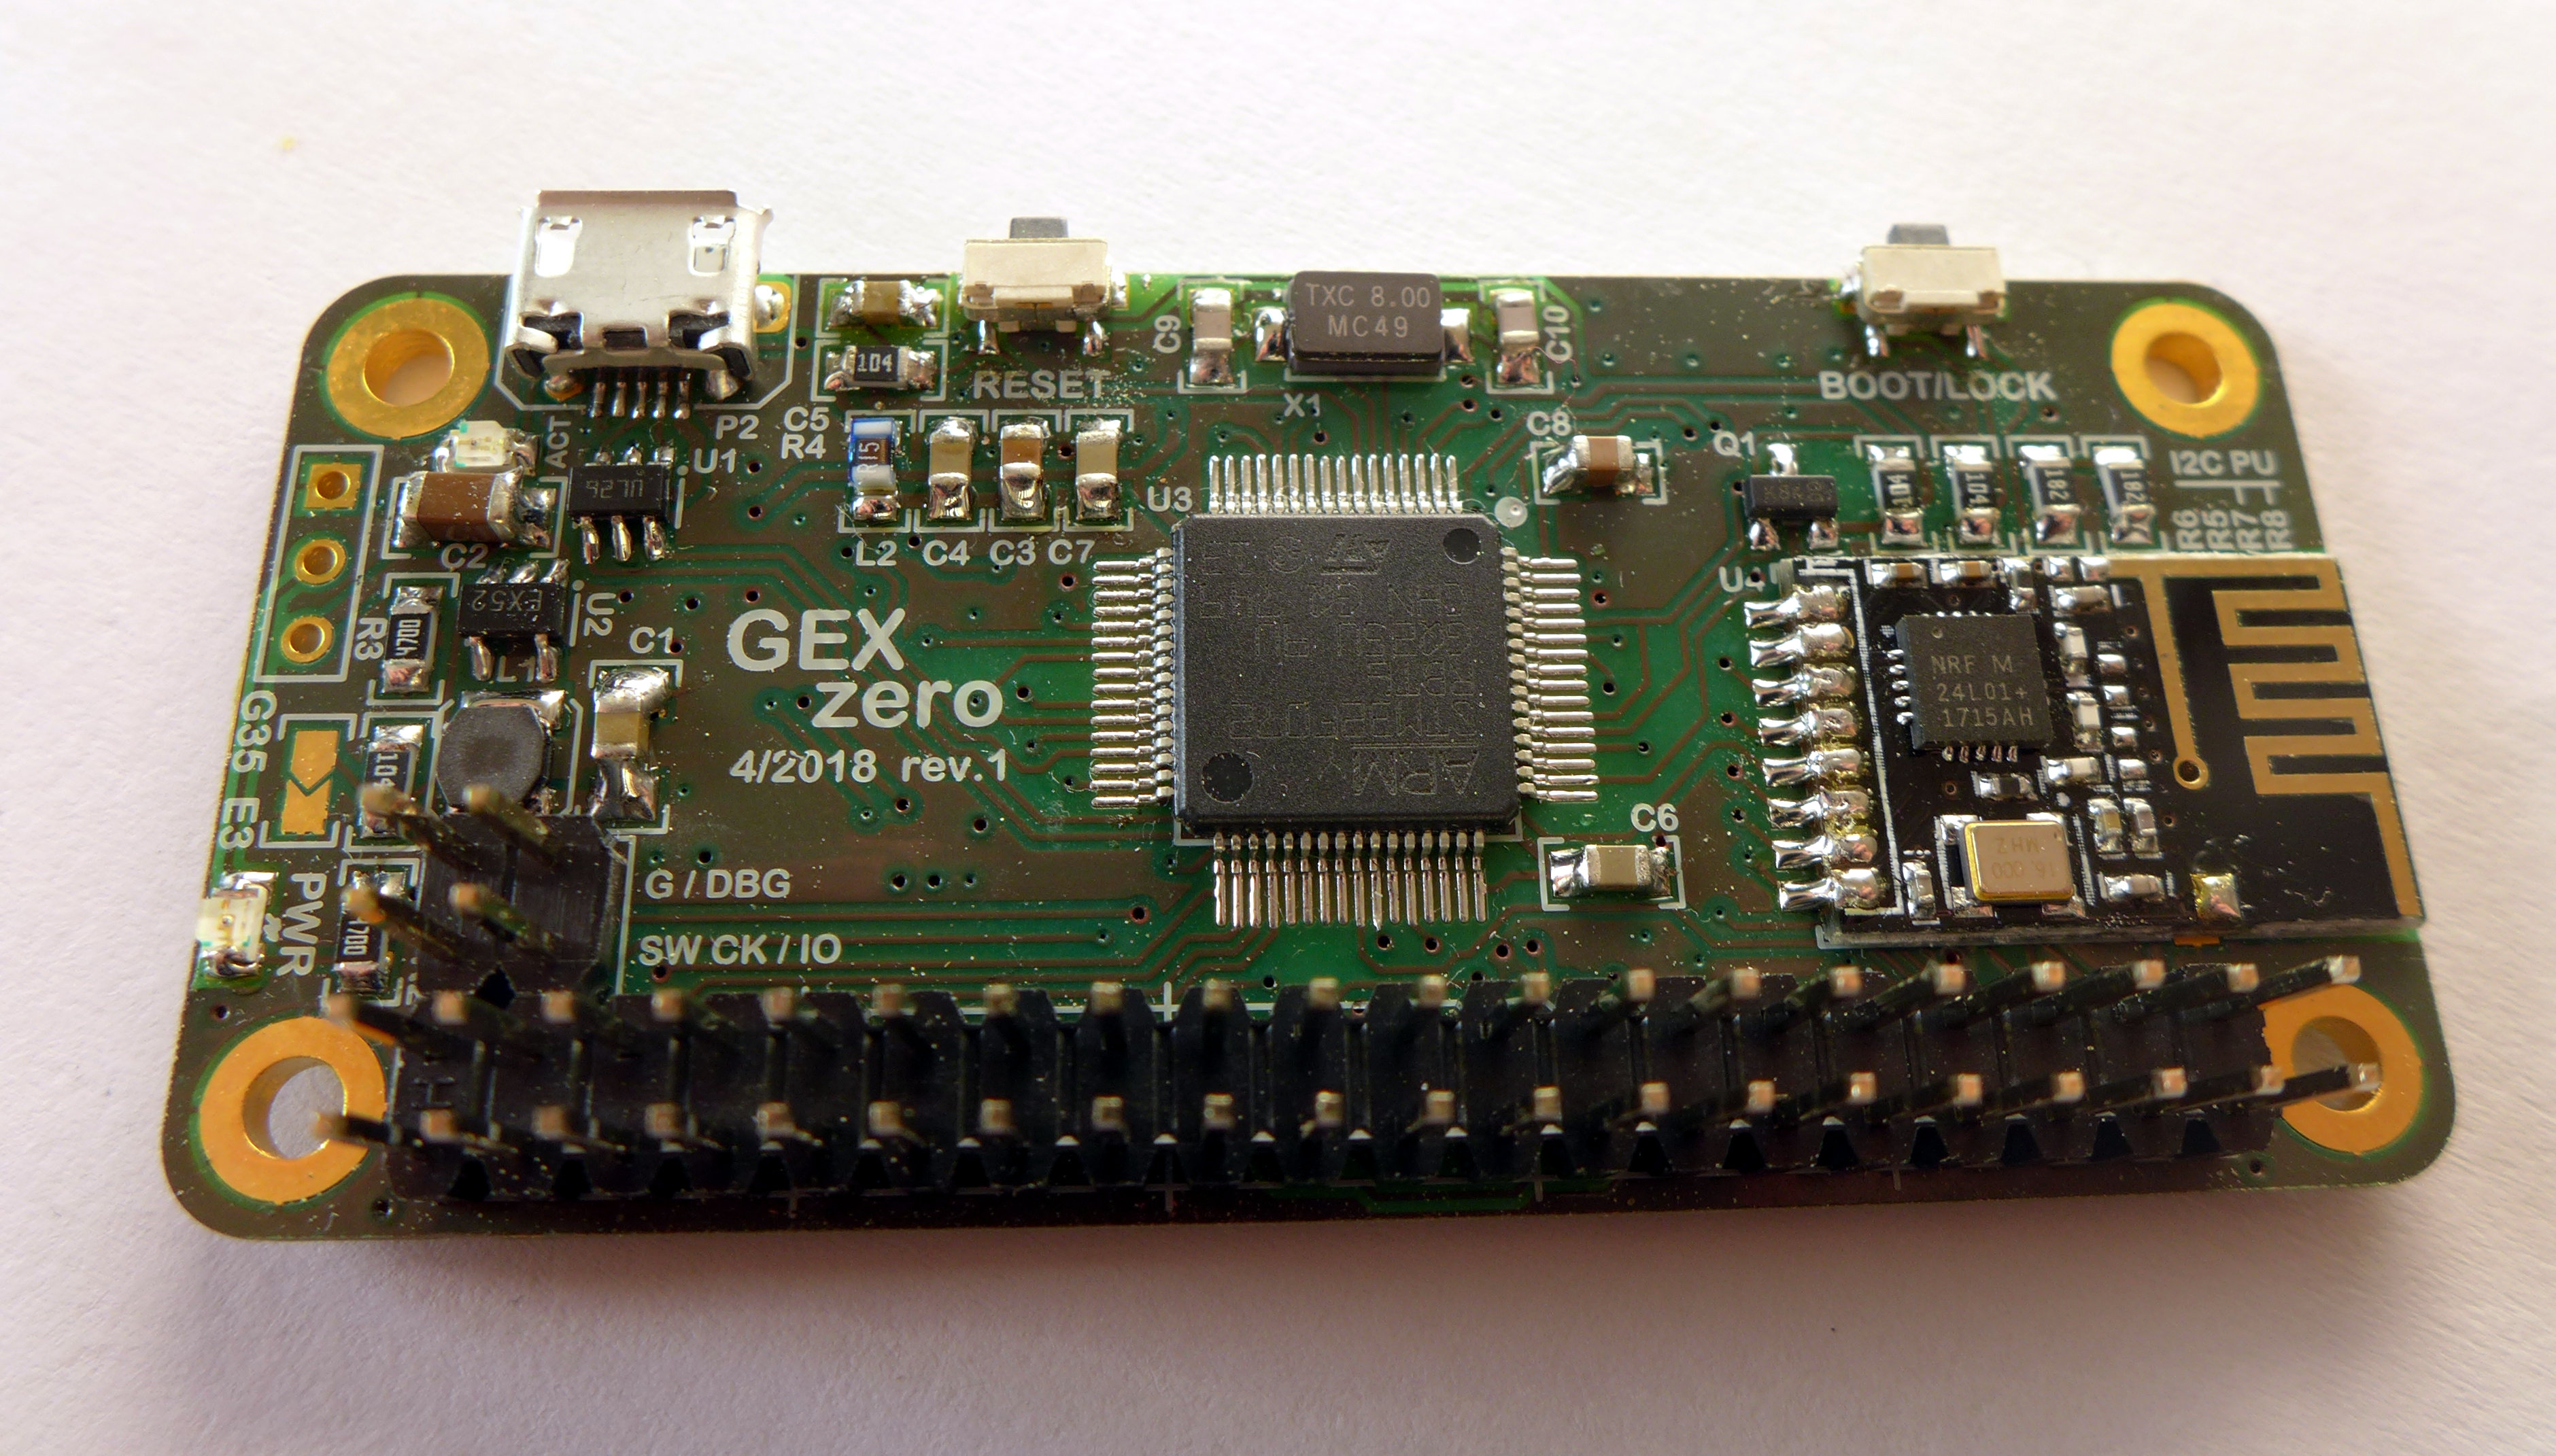
\includegraphics[width=.85\textwidth]{img/photo-zero-naked.jpg} \\
	%\vspace{1mm}
	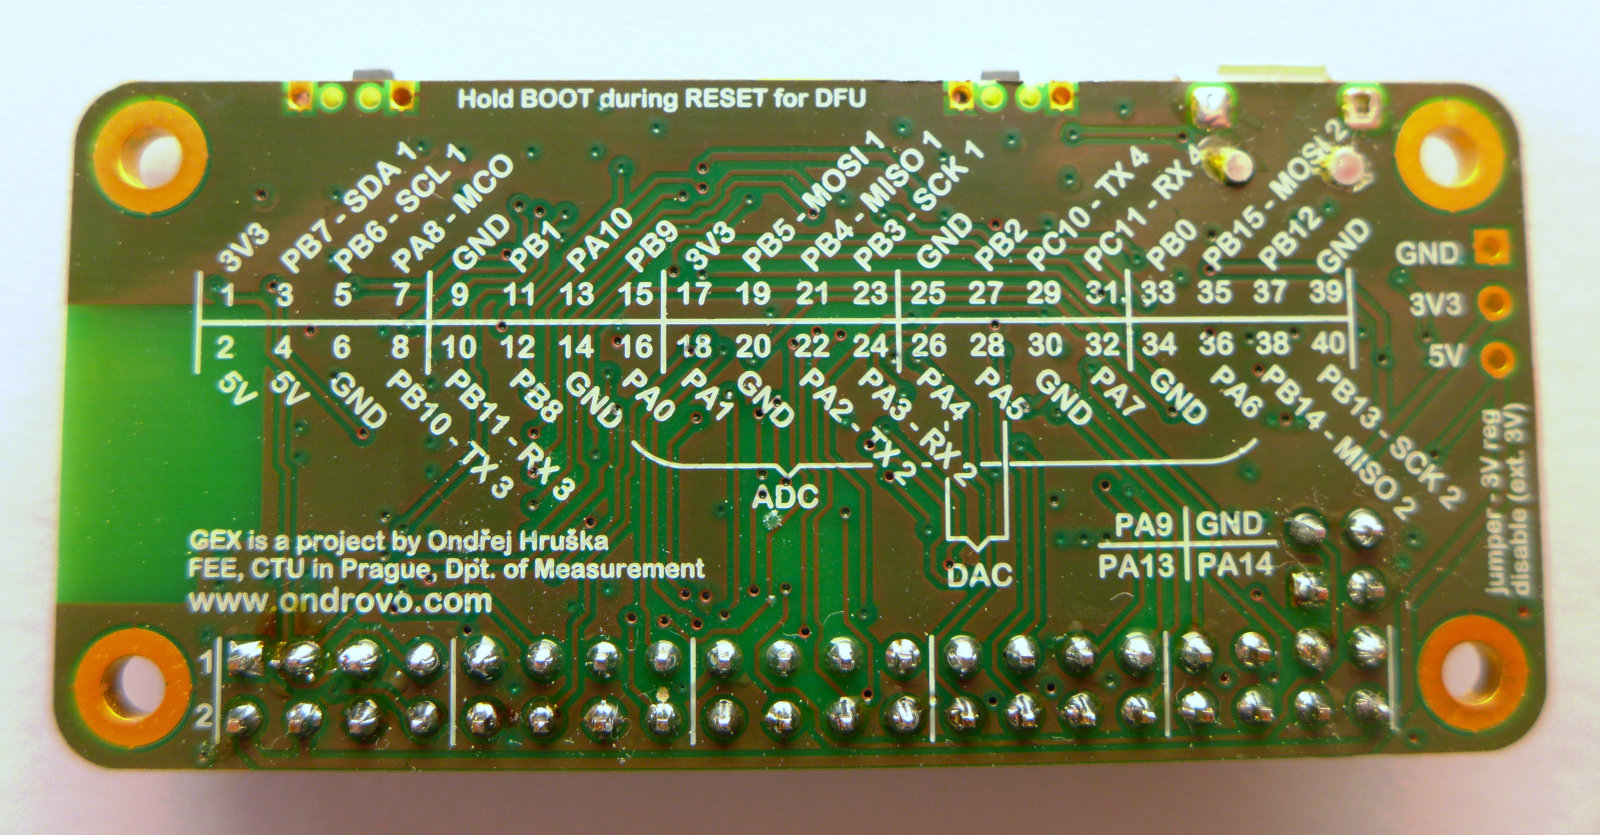
\includegraphics[width=.85\textwidth]{img/photo-zero-naked-bottom.jpg}
	\caption[GEX Zero back side]{\label{fig:gexz}Pin assignment diagram on the back side of GEX Zero}
\end{figure}

\iffalse
{
	\def\ptcw{.07\textwidth}
	\def\rpnl{\newline \footnotesize}
	\begin{table}[h]
		\begin{tabular}{
				W{\ptcw}W{\ptcw}W{\ptcw}W{\ptcw}|W{\ptcw}
				W{\ptcw}W{\ptcw}W{\ptcw}|W{\ptcw}W{\ptcw}
			}       
			\toprule
			\textbf{\color{blue}39} \rpnl
			GND
			&
			\textbf{37} \rpnl
			$\ast$
			&
			\textbf{35} \rpnl
			SPI\newline
			\null~MISO
			&
			\textbf{33} \rpnl
			PWM
			&
			\textbf{31} \rpnl
			$\ast$
			&
			\textbf{29} \rpnl
			$\ast$
			&
			\textbf{27} \rpnl
			\IIC\newline
			\null~SDA
			&
			\textbf{\color{blue}25} \rpnl
			GND
			&
			\textbf{23} \rpnl
			SPI\newline
			\null~SCK
			&
			\textbf{21} \rpnl
			SPI\newline
			\null~MISO
			\\
			\midrule
			\textbf{40} \rpnl
			SPI\newline
			\null~SCK
			&
			\textbf{38} \rpnl
			SPI\newline
			\null~MOSI
			&
			\textbf{36} \rpnl
			UART\newline
			\null~CTS
			&
			\textbf{\color{blue}34} \rpnl
			GND
			&
			\textbf{32} \rpnl
			PWM
			&
			\textbf{\color{blue}30} \rpnl
			GND
			&
			\textbf{28} \rpnl
			\IIC\newline
			\null~SCL
			&
			\textbf{26} \rpnl
			$\ast$
			&
			\textbf{24} \rpnl
			$\ast$
			&
			\textbf{22} \rpnl
			$\ast$   
			\\
			\bottomrule
		\end{tabular}
		\\[2mm]
		\begin{tabular}{
				W{\ptcw}W{\ptcw}|W{\ptcw}W{\ptcw}W{\ptcw}
				W{\ptcw}|W{\ptcw}W{\ptcw}W{\ptcw}W{\ptcw}
			}       
			\toprule
			\textbf{19} \rpnl
			SPI\newline
			\null~MOSI
			&
			\textbf{\color{red}17} \rpnl
			3.3\,V
			&
			\textbf{15} \rpnl
			$\ast$
			&
			\textbf{13} \rpnl
			$\ast$
			&
			\textbf{11} \rpnl
			UART\newline
			\null~RTS
			&
			\textbf{\color{blue}9} \rpnl
			GND
			&
			\textbf{7} \rpnl
			$\ast$
			&
			\textbf{5} \rpnl
			\IIC\newline
			\null~SCL
			&
			\textbf{3} \rpnl
			\IIC\newline
			\null~SDA
			&
			\textbf{\color{red}1} \rpnl
			3.3\,V
			\\
			\midrule
			\textbf{\color{blue}20} \rpnl
			GND
			&
			\textbf{18} \rpnl
			$\ast$
			&
			\textbf{16} \rpnl
			$\ast$
			&
			\textbf{\color{blue}14} \rpnl
			GND
			&
			\textbf{12} \rpnl
			PWM
			&
			\textbf{10} \rpnl
			UART\newline
			\null~RX
			&
			\textbf{8} \rpnl
			UART\newline
			\null~TX
			&
			\textbf{\color{blue}6} \rpnl
			GND
			&
			\textbf{\color{red}4} \rpnl
			5\,V
			&
			\textbf{\color{red}2} \rpnl
			5\,V
			\\      
			\bottomrule
		\end{tabular}
		\caption[Raspberry Pi GPIO header]{\label{tbl:pi_assignmenets}Raspberry Pi GPIO header (split into two lines), top view of the board, oriented with the USB connectors facing away from the user. ``$\ast$''~marks pins without important alternate functions.}
	\end{table}
}
\fi

The GEX Zero pin header's alternate functions had to match those on the RPi Zero header, so that the existing add-on boards can be used without modifications. By inspecting the alternate function tables in the STM32F072 datasheet~\cite{f072-ds}, we found a layout that fulfills this requirement almost perfectly. The final assignment is shown in \cref{tbl:gz_rpi_compare}, and the full schematic diagram is attached in \hyperref[apx:gex_zero]{Appendix B}.

\begin{table}
	\begin{tabularx}{\textwidth}{W{.1\textwidth}XX|W{.1\textwidth}XX}
		\toprule
		\textbf{Pin} & \textbf{RPi} & \textbf{GEX Zero} &
		\textbf{Pin} & \textbf{RPi} & \textbf{GEX Zero} \\
		
		\midrule
		\textbf{1} & \leavevmode\color{red}3.3\,V & -- &
		\textbf{2} & \leavevmode\color{red}5\,V & -- \\
		\textbf{3} & \IIC SDA & PB7 (SDA1) & 
		\textbf{4} & \leavevmode\color{red}5\,V & -- \\
		\textbf{5} & \IIC SCL & PB6 (SCL1) & 
		\textbf{6} & \leavevmode\color{blue}GND & -- \\
		\textbf{7} & $\ast$ & PA8 (MCO) & 
		\textbf{8} & UART TX & PB10 (TX3) \\
		
		\midrule
		\textbf{9} & \leavevmode\color{blue}GND & --
		& \textbf{10} & UART RX & PB11 (RX3) \\
		\textbf{11} & UART RTS & PB1 (RTS3)
		& \textbf{12} & PWM & PB8 \\
		\textbf{13} & $\ast$ & PA10 
		& \textbf{14} & \leavevmode\color{blue}GND & -- \\
		\textbf{15} & $\ast$ & PB9
		& \textbf{16} &  $\ast$ & PA0 (FCAP)\\
		
		\midrule
		\textbf{17} & \leavevmode\color{red}3.3\,V & --
		& \textbf{18} &  $\ast$ & PA1 \\
		\textbf{19} & SPI MOSI & PB5 (MOSI1)
		& \textbf{20} & \leavevmode\color{blue}GND & -- \\
		\textbf{21} & SPI MISO & PB4 (MISO1)
		& \textbf{22} &  $\ast$ & PA2 (TX2) \\
		\textbf{23} & SPI SCK & PB3 (SCK1)
		& \textbf{24} &  $\ast$ & PA3 (RX2) \\
		
		\midrule
		\textbf{25} & \leavevmode\color{blue}GND & --
		& \textbf{26} &  $\ast$ & PA4 (DAC$_1$) \\
		\textbf{27} & ID \IIC SDA & PB2 
		& \textbf{28} & ID \IIC SCL & PA5 (DAC$_2$) \\
		\textbf{29} & $\ast$ & PC10 (TX4)
		& \textbf{30} & \leavevmode\color{blue}GND & -- \\
		\textbf{31} & $\ast$ & PC11 (RX4)
		& \textbf{32} & PWM & PA7 \\
		
		\midrule
		\textbf{33} & PWM & PB0 
		& \textbf{34} & \leavevmode\color{blue}GND & -- \\
		\textbf{35} & SPI MISO & PB14~(MISO2)
		& \textbf{36} &  $\ast$ & PA6 (CTS3) \\
		\textbf{37} & $\ast$ & PB12
		& \textbf{38} & SPI MOSI & PB15~(MOSI2)\\
		\textbf{39} & \leavevmode\color{blue}GND & -- 
		& \textbf{40} & SPI SCK & PB13 (SCK2)\\
		\bottomrule 
	\end{tabularx}
	\caption[Comparison of the RPI Zero and GEX Zero GPIO headers]{\label{tbl:gz_rpi_compare}
		Comparison of the RPi Zero and GEX Zero GPIO header pin assignments. Names in parentheses represent STM32F072 alternate functions (e.g., MISO1 is MISO of the first SPI peripheral). ``$\ast$''~marks pins without important alternate functions that could be assigned arbitrarily in the GEX Zero header. All power pins are identical in both headers.
	}
\end{table}

\gls{GPIO} ports A and B are fully exposed in the header, with the exception of pins PA11 and PA12 that are routed to the USB connector. The remaining positions were filled pith pins from port C. The omitted ``ID \IIC'' port on pins 27 and 28 is used by the RPi Zero to read configuration from an EEPROM chip on some add-on boards. As this is the only use of the \IIC port, its lack is not a big limitation.

\section{GEX Zero Errata}

The GEX Hub \gls{PCB} had to be updated to correct some layout mistakes.
Unfortunately, neither GEX Zero \gls{PCB} was flawless in the first revision. The errors should not interfere much in the usage of the module; nonetheless, they were fixed in the schematic for any future production of the board.

\begin{itemize}
	\item The \IIC pull-up resistor R8 is connected to PA8 instead of PB7. This can be fixed by cutting the trace near the \gls{GPIO} header and rewiring it, or using an external 1.8\,k$\Omega$ pull-up resistor on PB7, when the \IIC connection is required.
	\item Pins PB14 and PB15 are swapped in the \gls{GPIO} header, making the SPI port incompatible with add-on boards using this interface. Luckily, there is another SPI port on the header, which is routed correctly, somewhat mitigating this mistake.
\end{itemize}

\section{Wireless Gateway} \label{sec:rfgateway}

The wireless gateway was designed as a ``\gls{USB} dongle'', using the \gls{USB} type A connector (\cref{fig:gwxgw}). It is fitted with an STM32F103 microcontroller, selected for its low cost and availability in small packages (in this case LQFP48)\footnote{ Ironically, the STM32F103 is more powerful than the \gls{MCU} used in GEX Zero and GEX Hub. Porting GEX to this platform is planned for future development.}. The nRF24L01+ module is partly sticking outside the board outline, allowing the \gls{PCB} to be smaller (and thus cheaper to manufacture), while reducing interference between components and copper plating on the board and the antenna. The schematic diagram of the wireless gateway is attached in \hyperref[apx:gex_wgw]{Appendix C}.

Beyond the use with GEX, the gateway is a versatile tool which could be programmed with a different firmware and serve other purposes, e.g., as a wireless connection between two computers, to scan the radio spectrum for interference in order to find a clear channel, or to communicate with other devices that use the nRF24L01+ transceiver. The chosen microcontroller, unfortunately, does not include a USB bootloader, so a SWD programmer is required to change the firmware; SWD is routed to the pin header next to the wireless module.


\begin{figure}[h]
	\centering
	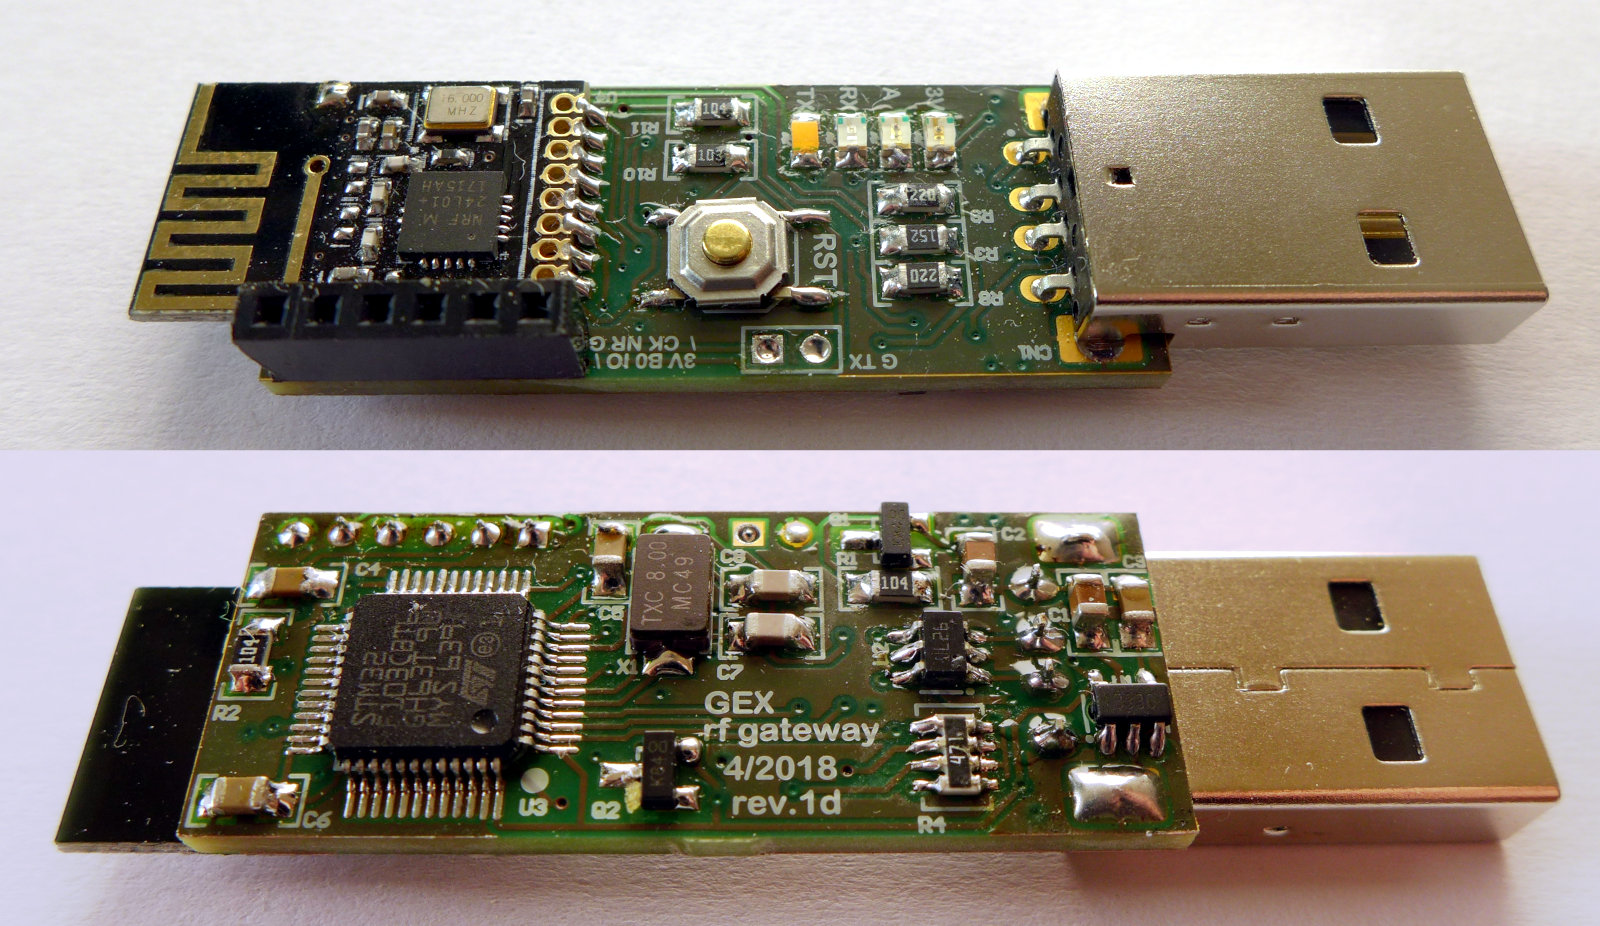
\includegraphics[width=.9\textwidth]{img/photo-rfdongle.jpg}
	\caption{\label{fig:gwxgw}The wireless gateway (top and bottom side)}
\end{figure}
